\documentclass[11pt,a4paper]{article}
\usepackage[utf8]{inputenc}
\usepackage[T1]{fontenc}
\renewcommand{\contentsname}{Table des matières}
\usepackage{amsmath,amssymb}
\usepackage{geometry}
\geometry{margin=2.2cm}
\usepackage{tikz}
\usetikzlibrary{arrows.meta,calc}
\usepackage{xcolor}
\usepackage{enumitem}
\usepackage{booktabs}
\usepackage{tabularx}
\usepackage{mdframed}
\usepackage{hyperref}
\hypersetup{colorlinks=true,linkcolor=blue!50!black,urlcolor=blue}

% ---- boîtes personnalisées ----
\newmdenv[
  linecolor=blue!60!black, backgroundcolor=blue!4,
  linewidth=1pt, roundcorner=4pt, innermargin=8pt, innertopmargin=8pt, innerbottommargin=8pt,
  skipabove=8pt, skipbelow=8pt
]{methode}

\newmdenv[
  linecolor=orange!70!black, backgroundcolor=orange!6,
  linewidth=1pt, roundcorner=4pt, innermargin=8pt, innertopmargin=8pt, innerbottommargin=8pt,
  skipabove=8pt, skipbelow=8pt
]{piege}

\newmdenv[
  linecolor=black!60, backgroundcolor=black!3,
  linewidth=0.8pt, roundcorner=3pt, innermargin=8pt, innertopmargin=6pt, innerbottommargin=6pt,
  skipabove=8pt, skipbelow=8pt
]{enonce}

\newmdenv[
  linecolor=green!45!black, backgroundcolor=green!5,
  linewidth=1pt, roundcorner=4pt, innermargin=8pt, innertopmargin=6pt, innerbottommargin=6pt,
  skipabove=6pt, skipbelow=10pt
]{correction}

\newcommand{\eqbox}[1]{\[\boxed{#1}\]}

\title{\textbf{Préparation examen -- Mécathermo}\\[4pt]\large Guide de résolution, fiches méthode \& exercices corrigés}
\author{}
\date{}

\begin{document}
\maketitle
\vspace{-1.2cm}
\begin{center}
\small\itshape Basé sur le syllabus « Mise à niveau thermodynamique » et les exercices supplémentaires du cours.\\
Le formulaire officiel est autorisé à l'examen : ce document donne la \emph{méthode} pour l'utiliser efficacement.
\end{center}
\vspace{0.4cm}

\tableofcontents
\newpage

\section{Méthode générale de résolution}

Les exercices d'examen sont presque toujours un \textbf{cycle} (moteur, frigo/PAC) ou une \textbf{suite de
transformations} d'un gaz ou d'un fluide. La méthode ci-dessous fonctionne dans tous les cas : elle consiste
à remplir un \emph{tableau d'état} point par point, puis à appliquer les principes de la thermo transformation
par transformation. C'est la même logique que celle utilisée partout dans le syllabus (moteurs, frigo, cycles
industriels).

\begin{methode}
\textbf{Les 6 étapes, dans l'ordre}
\begin{enumerate}[label=\textbf{\arabic*.}, leftmargin=1.6em]
\item \textbf{Dessiner le schéma du système} (ouvert/fermé) et le \textbf{cycle en diagramme $p$-$V$} (ou
$\log p$-$h$ pour un frigo). Identifier chaque transformation : isobare, isochore, isotherme, adiabatique
réversible.
\item \textbf{Numéroter/lettrer les points} (comme dans le cours : A,B,C,... ou 1,2,3,...) et faire un
\textbf{tableau} avec une colonne par point et une ligne par grandeur ($p$, $V$, $T$, $n$ ou $m$).
\item \textbf{Remplir ce que l'énoncé donne directement}, puis \textbf{propager} à l'aide des lois de
transformation (tableau ci-dessous) jusqu'à avoir $p,V,T$ en chaque point.
\item \textbf{Calculer $W$ et $Q$ pour chaque transformation} (formules ci-dessous), en respectant les signes.
\item \textbf{Sommer sur le cycle} : $W_{cycle}=\sum W_i$, $Q_{cycle}=\sum Q_i$ (doit donner $\Delta U_{cycle}=0$,
c'est une bonne vérification).
\item \textbf{Répondre à la question posée} : rendement, COP/PSN, puissance, débit, etc. -- toujours en
reliant à $W$ et $Q$ déjà calculés.
\end{enumerate}
\end{methode}

\subsection{Reconnaître le type de transformation}

\begin{center}
\renewcommand{\arraystretch}{1.4}
\begin{tabularx}{\linewidth}{@{}l l X@{}}
\toprule
\textbf{Transfo} & \textbf{Loi} & \textbf{Comment la reconnaître dans l'énoncé} \\
\midrule
Isobare ($p$=cste) & $V/T=$cste & « admission/échappement », « échangeur (condenseur/évaporateur) »,
« combustion diesel », chauffage/refroidissement dans un circuit ouvert \\
Isochore ($V$=cste) & $p/T=$cste & « explosion » (essence), soupapes fermées à volume bloqué, chute de
pression à l'échappement \\
Isotherme ($T$=cste) & $pV=$cste & rare dans ce cours (Carnot théorique) \\
Adiabatique réversible & $pV^\gamma=$cste \quad $TV^{\gamma-1}=$cste \quad $T^\gamma V^{1-\gamma}=$cste
& compression/détente \textbf{rapide} : compresseur, turbine, compression/détente dans un cylindre
(pas le temps d'échanger de la chaleur) \\
Isenthalpique ($h$=cste) & $h=$cste & détente dans une \textbf{soupape/vanne de détente} (frigo) \\
Isentropique & $s$=cste & compression \textbf{réversible} dans un compresseur frigo (1-2) \\
\bottomrule
\end{tabularx}
\end{center}

\begin{piege}
\textbf{Piège classique} : ne pas confondre une adiabatique \emph{réversible} ($pV^\gamma=$cste, utilisable
seulement ici) avec une adiabatique quelconque ($Q=0$ mais pas forcément cette loi). Dans ce cours, sauf
mention contraire, toute compression/détente « rapide » est supposée adiabatique réversible.
\end{piege}

\subsection{Les deux versions du 1\textsuperscript{er} principe}

\begin{center}
\renewcommand{\arraystretch}{1.5}
\begin{tabularx}{\linewidth}{@{}l l X@{}}
\toprule
\textbf{Système} & \textbf{Formule} & \textbf{Quand l'utiliser} \\
\midrule
\textbf{Fermé} (cylindre, gaz enfermé) & $\Delta U = W + Q$ \quad avec $dU=nC_v\,dT$ &
Moteurs à piston (cycle B-C-D-E dans le cylindre) \\
\textbf{Ouvert} (fluide qui traverse une machine) & $\Delta H = W_{ut} + Q$ \quad avec $dH=nC_p\,dT$ &
Compresseur, turbine, échangeur, soupape de détente (frigo, cycles à débit) \\
\bottomrule
\end{tabularx}
\end{center}

\begin{piege}
\textbf{Erreur n°1 à l'examen} : utiliser $C_v$ dans un système ouvert (ou l'inverse). Règle simple :
\emph{ça coule dans un tuyau/une machine à débit} $\Rightarrow$ ouvert $\Rightarrow$ $H$ et $C_p$.
\emph{C'est enfermé dans un cylindre/récipient} $\Rightarrow$ fermé $\Rightarrow$ $U$ et $C_v$.
\end{piege}

\subsection{Travail et chaleur transformation par transformation}

\begin{center}
\renewcommand{\arraystretch}{1.6}
\begin{tabularx}{\linewidth}{@{}l X X@{}}
\toprule
& \textbf{Système fermé} ($W=-\int p\,dV$) & \textbf{Système ouvert} ($W_{ut}$) \\
\midrule
Isobare & $W=-p\Delta V$, \ $Q=nC_v\Delta T + p\Delta V = nC_p\Delta T\ (\text{si } \Delta U{=}nC_v\Delta T)$ &
$W_{ut}=0$ (pas de pièce mobile utile), \ $Q=\Delta H = nC_p\Delta T$ \\
Isochore & $W=0$, \ $Q=\Delta U = nC_v\Delta T$ & (n'existe pas en ouvert : pas de sens physique) \\
Adiabatique rév. & $Q=0$, \ $W=\Delta U = nC_v\Delta T$ & $Q=0$, \ $W_{ut}=\Delta H = nC_p\Delta T$
(compresseur/turbine) \\
Isenthalpique & -- & $\Delta H=0 \Rightarrow Q=-W_{ut}$ ; soupape de détente : $W_{ut}=0 \Rightarrow Q=0$
donc $h$ constante \\
\bottomrule
\end{tabularx}
\end{center}

\subsection{Conventions de signe (à respecter tout le temps)}

\begin{itemize}[leftmargin=1.4em]
\item Énergie \textbf{reçue} par le système (chaleur ou travail) $\rightarrow$ \textbf{positive}.
\item Énergie \textbf{cédée} par le système $\rightarrow$ \textbf{négative}.
\item Un \textbf{cycle moteur} (tourne dans le sens horaire sur le diagramme $p$-$V$) \textbf{fournit} du
travail à l'extérieur $\Rightarrow$ $W_{cycle}<0$.
\item Un \textbf{cycle récepteur} (frigo, PAC -- sens antihoraire) \textbf{reçoit} du travail
$\Rightarrow$ $W_{cycle}>0$.
\item Toujours travailler en \textbf{Kelvin} pour les lois des gaz et les rapports adiabatiques.
\end{itemize}

\subsection{Rendements et coefficients -- à ne jamais confondre}

\begin{center}
\renewcommand{\arraystretch}{1.6}
\begin{tabularx}{\linewidth}{@{}l X@{}}
\toprule
\textbf{Grandeur} & \textbf{Définition} \\
\midrule
$\eta_{\text{théorique}}$ & $\dfrac{|W_{\text{théorique}}|}{Q_{CD}}$ -- rendement du cycle idéal (courbes théoriques
p-V), ne dépend que de $\varepsilon$ (et $\rho$ pour le diesel) \\
$\eta_{forme}=\eta_f$ & $\dfrac{|W_{\text{indiqué}}|}{|W_{\text{théorique}}|}$ -- pertes car le cycle réel ne suit pas
exactement les courbes théoriques (combustion non instantanée, refroidissement parois, pertes de charge) \\
$\eta_{\text{méca}}$ & $\dfrac{|W_{disponible}|}{|W_{\text{indiqué}}|}$ -- pertes par frottements mécaniques \\
$\eta_{eff}$ & $\eta_{th}\cdot\eta_f\cdot\eta_{\text{méca}}=\dfrac{|W_{disponible}|}{Q_{CD}}$ -- rendement global,
$Q_{CD}=m_{carburant}\cdot PCI$ \\
$COP$ (pompe à chaleur) & $\dfrac{-Q_1}{W}$ -- énergie utile = chaleur cédée à la source chaude \\
$PSN$ (frigo) & $\dfrac{Q_2}{W}$ -- énergie utile = chaleur prise à la source froide \\
$\eta_{Carnot}/COP_{max}/PSN_{max}$ & bornes théoriques \emph{réversibles} entre $T_1$ (chaude) et $T_2$
(froide) : $\eta_{Carnot}=1-\dfrac{T_2}{T_1}$, \ $COP_{max}=\dfrac{T_1}{T_1-T_2}$, \
$PSN_{max}=\dfrac{T_2}{T_1-T_2}$ \\
\bottomrule
\end{tabularx}
\end{center}

\begin{piege}
Un rendement \textbf{ne se calcule presque jamais directement} : c'est toujours un \textbf{rapport de deux
travaux/chaleurs} que vous avez calculés à l'étape 4-5 de la méthode. Ne cherchez pas une « formule magique »
sans être passé par le tableau d'état.
\end{piege}

\subsection{Check-list avant de rendre une copie}
\begin{itemize}[leftmargin=1.4em]
\item Toutes les températures sont-elles en Kelvin ?
\item Le signe de $W$ et $Q$ est-il cohérent avec le sens du cycle (moteur $\to$ négatif, récepteur $\to$
positif) ?
\item $\Delta U_{cycle}=0$ et $\Delta H_{cycle}=0$ ont-ils été vérifiés (somme des transformations) ?
\item Le rendement trouvé est-il \textbf{physiquement raisonnable} (entre 0 et $\eta_{Carnot}$ pour un moteur,
$COP>1$ pour une PAC) ?
\item Les unités sont-elles cohérentes (J vs kJ, bar vs Pa) ?
\end{itemize}

\newpage
\section{Fiche : moteurs à combustion (essence, diesel, 2 temps)}

\subsection{Les 3 cycles -- vue d'ensemble}

Dans les trois cas, le cycle réel du cylindre (fermé, gaz emprisonné) est le même \textbf{cycle utile}
B-C-D-E-B ; les temps d'admission (A-B) et d'échappement (B-A), tous deux isobares à $p_{atm}$, s'annulent
en travail net et ne comptent pas dans le rendement. Seule la nature de la combustion (isochore ou isobare)
change.

\begin{center}
\small
\renewcommand{\arraystretch}{1.5}
\begin{tabularx}{\linewidth}{@{}>{\raggedright\arraybackslash}p{2.5cm} *{3}{>{\raggedright\arraybackslash}X}@{}}
\toprule
& \textbf{Essence (B. de Rochas)} & \textbf{Diesel} & \textbf{2 temps} \\
\midrule
Admission A-B & isobare (air+essence) & isobare (air seul) & isobare (via lumières) \\
Compression B-C & adiabatique rév. & adiabatique rév. ($\varepsilon$ plus grand) & adiabatique rév. \\
Combustion C-D & \textbf{isochore} (explosion, bougie) & \textbf{isobare} (injection + auto-inflammation) &
isochore \\
Détente D-E & adiabatique rév. & adiabatique rév. & adiabatique rév. \\
Échappement E-B puis B-A & isochore puis isobare & isochore puis isobare & isochore/isobare via lumières \\
$\varepsilon=V_B/V_A=V_B/V_C$ & $8<\varepsilon<10$ & $16<\varepsilon<20$ & variable \\
Tours moteur / cycle & 2 tours & 2 tours & \textbf{1 tour} \\
\bottomrule
\end{tabularx}
\end{center}

\begin{center}
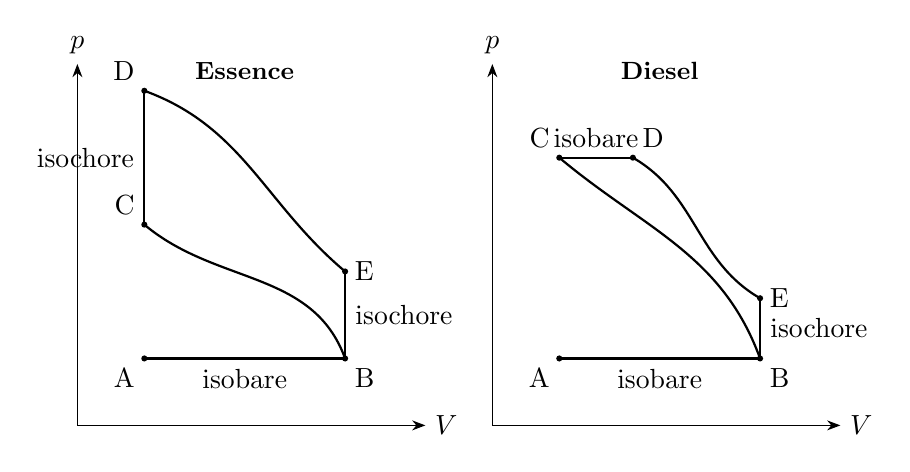
\begin{tikzpicture}[scale=0.85, >=Stealth]
% --- Essence ---
\begin{scope}
\draw[->] (0,0) -- (5.2,0) node[right] {$V$};
\draw[->] (0,0) -- (0,5.4) node[above] {$p$};
\coordinate (A) at (1,1); \coordinate (B) at (4,1);
\coordinate (C) at (1,3); \coordinate (D) at (1,5);
\coordinate (E) at (4,2.3);
\draw[thick] (A) -- (B) node[midway,below]{isobare};
\draw[thick] (B) to[out=110,in=-40] (C);
\draw[thick] (C) -- (D) node[midway,left]{isochore};
\draw[thick] (D) to[out=-20,in=140] (E);
\draw[thick] (E) -- (B) node[midway,right]{isochore};
\draw[thick,dashed] (B) -- (A) ;
\foreach \p/\lab/\pos in {A/A/below left,B/B/below right,C/C/above left,D/D/above left,E/E/right}
  {\fill (\p) circle (1.3pt) node[\pos] {\lab};}
\node at (2.5,5.3) {\small\bfseries Essence};
\end{scope}
% --- Diesel ---
\begin{scope}[xshift=6.2cm]
\draw[->] (0,0) -- (5.2,0) node[right] {$V$};
\draw[->] (0,0) -- (0,5.4) node[above] {$p$};
\coordinate (A) at (1,1); \coordinate (B) at (4,1);
\coordinate (C) at (1,4); \coordinate (D) at (2.1,4);
\coordinate (E) at (4,1.9);
\draw[thick] (A) -- (B) node[midway,below]{isobare};
\draw[thick] (B) to[out=110,in=-40] (C);
\draw[thick] (C) -- (D) node[midway,above]{isobare};
\draw[thick] (D) to[out=-30,in=150] (E);
\draw[thick] (E) -- (B) node[midway,right]{isochore};
\draw[thick,dashed] (B) -- (A);
\foreach \p/\lab/\pos in {A/A/below left,B/B/below right,C/C/above left,D/D/above right,E/E/right}
  {\fill (\p) circle (1.3pt) node[\pos] {\lab};}
\node at (2.5,5.3) {\small\bfseries Diesel};
\end{scope}
\end{tikzpicture}
\end{center}

\begin{piege}
Le rendement \textbf{théorique} d'un moteur ne dépend \emph{jamais} du carburant ni de la puissance : il ne
dépend que de la \textbf{géométrie} ($\varepsilon$, et $\rho$ pour le diesel) et de $\gamma$. C'est souvent
la première sous-question et elle se résout \textbf{sans aucune donnée sur la combustion}.
\end{piege}

\subsection{Formules essentielles}

\begin{center}
\renewcommand{\arraystretch}{1.7}
\begin{tabularx}{\linewidth}{@{}l X@{}}
\toprule
Rapport volumétrique & $\varepsilon = \dfrac{V_B}{V_A}=\dfrac{V_B}{V_C}$ \\
Rapport de combustion (diesel) & $\rho = \dfrac{V_D}{V_C}$ \\
$\eta_{\text{théo}}$ essence & $\eta_{\text{théo}}=1-\varepsilon^{1-\gamma}$ \\
$\eta_{\text{théo}}$ diesel & $\eta_{\text{théo}}=1+\dfrac{\varepsilon^{1-\gamma}-\varepsilon^{1-\gamma}\rho^\gamma}
{\gamma(\rho-1)}$ \\
Chaleur apportée & $Q_{CD}=m_{carburant}\cdot PCI$ (isochore essence : $Q_{CD}=nC_v(T_D-T_C)$ ; isobare
diesel : $Q_{CD}=nC_p(T_D-T_C)$) \\
Rendements en cascade & $\eta_{eff}=\eta_{\text{théo}}\cdot\eta_{f}\cdot\eta_{\text{méca}}=\dfrac{|W_{disponible}|}{Q_{CD}}$ \\
Puissance (4 temps, $z$ cylindres) & $P=\dfrac{N}{2\cdot 60}\cdot W\cdot z$ \quad ($N$ en tr/min, 1 cycle =
2 tours) \\
Puissance (2 temps) & $P=\dfrac{N}{60}\cdot W\cdot z$ \quad (1 cycle = 1 tour) \\
Pression moyenne indiquée & $W_{réel}=pmi\cdot(V_A-V_B)=pmi\cdot\pi r^2 x$ ($x$=course), $pmi=p_M-p_{atm}$ \\
Combustion hydrocarbure & $C_xH_y+\left(x+\dfrac{y}{4}\right)O_2 \to xCO_2+\dfrac{y}{2}H_2O$ +chaleur \\
Excès d'air & $\lambda=\dfrac{\text{air réellement aspiré}}{\text{air stœchiométrique}}$ (essence
$\lambda\approx 1$, diesel souvent $\lambda>1$) \\
\bottomrule
\end{tabularx}
\end{center}

\begin{piege}
Ne confondez pas $V_A$ et $V_C$ : $V_A$ (avant admission) $=V_C$ (fin de compression) $=$ volume mort
(point mort haut, PMH). $V_B$ (fin d'admission) $=$ point mort bas (PMB). La cylindrée $=V_B-V_A$.
\end{piege}

\newpage
\subsection{Exemple complet résolu -- moteur essence 4 cylindres}

\begin{enonce}
Moteur essence 4 temps, 4 cylindres, cylindrée totale $1{,}2$ L ($0{,}3$ L/cylindre). Rapport volumétrique
$\varepsilon=10$. Puissance effective $P_{eff}=20$ kW. Air aspiré : $16\,^\circ\text{C}$, $1$ bar, gaz
parfait, $\gamma=1{,}4$, $21\%$ O$_2$ en volume. Carburant simplifié CH$_{1,8}$, excès d'air
$\lambda=1{,}2$, PCI $=42500$ kJ/kg. $\eta_{\text{méca}}=0{,}8$, $\eta_{forme}=0{,}75$.

\emph{Trouver : $T,p,V$ en chaque point, le rendement théorique, et la vitesse de rotation du moteur.}
\end{enonce}

\begin{correction}
\textbf{1) Tableau des volumes.} Cylindrée $=V_B-V_A=300\text{ cm}^3$ et $\varepsilon=V_B/V_A=10$
$\Rightarrow 9V_A=300 \Rightarrow V_A=V_C=33{,}3\text{ cm}^3$, \ $V_B=333{,}3\text{ cm}^3$.

\textbf{2) Point B} (fin d'admission = air ambiant) : $T_B=289{,}15$ K, $p_B=1$ bar.

\textbf{3) Compression B$\to$C (adiabatique réversible)} :
\[T_C=T_B\,\varepsilon^{\gamma-1}=289{,}15\cdot 10^{0{,}4}=726{,}3\text{ K}\qquad
p_C=p_B\,\varepsilon^{\gamma}=10^{1{,}4}=25{,}1\text{ bar}\]

\textbf{4) Rendement théorique} (ne dépend que de $\varepsilon,\gamma$) :
\eqbox{\eta_{\text{théo}}=1-\varepsilon^{1-\gamma}=1-10^{-0{,}4}=1-0{,}3981=0{,}6019=\mathbf{60{,}2\%}}

\textbf{5) Masse de carburant par cycle et par cylindre.} Réaction : $CH_{1,8}+1{,}45\,O_2 \to CO_2+0{,}9H_2O$,
donc $1{,}45$ mol O$_2$/mol carburant, soit $\dfrac{1{,}45}{0{,}21}=6{,}905$ mol air stœchiométrique par mol
carburant. Avec $\lambda=1{,}2$ : $6{,}905\times 1{,}2=8{,}29$ mol air réel / mol carburant.

Moles totales dans le cylindre en B (mélange air+carburant, gaz parfait) :
\[n_{mix}=\frac{p_BV_B}{RT_B}=\frac{10^5\times 333{,}3\times10^{-6}}{8{,}314\times 289{,}15}=0{,}01386\text{ mol}\]
Avec $n_{mix}=n_{carb}(8{,}29+1)$ : $n_{carb}=1{,}49\times10^{-3}$ mol $\Rightarrow$
$m_{carb}=n_{carb}\times M_{CH_{1,8}}=1{,}49\times10^{-3}\times13{,}8=2{,}06\times10^{-5}$ kg.

\textbf{6) Chaleur et travaux (par cylindre, par cycle).}
\[Q_{CD}=m_{carb}\cdot PCI = 2{,}061\times10^{-5}\times 42{,}5\times10^{6}=875{,}8\text{ J}\]
\[|W_{\text{théo}}|=\eta_{\text{théo}}\cdot Q_{CD}=0{,}6019\times875{,}8=527{,}1\text{ J}\]
\[|W_{\text{indiqué}}|=\eta_f\cdot|W_{\text{théo}}|=0{,}75\times527{,}1=395{,}4\text{ J} \qquad
|W_{disponible}|=\eta_{\text{méca}}\cdot|W_{\text{indiqué}}|=0{,}8\times395{,}4=316{,}3\text{ J}\]

\textbf{7) Vitesse de rotation.} $P_{eff}=\dfrac{N}{2\cdot 60}\cdot|W_{disponible}|\cdot z$ avec $z=4$ :
\eqbox{N=\frac{P_{eff}\cdot 120}{|W_{disponible}|\cdot z}=\frac{20\,000\times120}{316{,}3\times4}
= \mathbf{1897\ \text{tr/min}}}

\emph{(Le corrigé du cours annonce 1881 tr/min : l'écart de $0{,}8\ \%$ vient de ses arrondis
intermédiaires. Le calcul ci-dessus boucle exactement, cf. la vérification $\sum Q+\sum W=0$.)}

\emph{(Le tableau complet $T_D,p_D,T_E,p_E$ s'obtient ensuite : $T_D$ via $Q_{CD}=nC_v(T_D-T_C)$ à $V$
constant avec $n=n_{mix}$, puis $D\to E$ adiabatique jusqu'à $V_E=V_B$, exactement comme à l'étape 3.)}
\end{correction}

\newpage
\section{Fiche : machines frigorifiques / pompes à chaleur (ex. R134a)}

\subsection{Principe et schéma}

Un frigo et une pompe à chaleur (PAC) sont la \textbf{même machine} : un \textbf{cycle récepteur} à deux
sources (il faut fournir du travail $W>0$ au fluide). Seule change l'énergie « utile » :
\begin{itemize}[leftmargin=1.4em]
\item \textbf{Frigo} : utile $=Q_2$ (chaleur \emph{prise} à la source froide, l'intérieur du frigo).
\item \textbf{PAC} : utile $=-Q_1$ (chaleur \emph{cédée} à la source chaude, l'intérieur de la maison) ;
la chaleur prise à la source froide (air extérieur) est considérée \textbf{gratuite}.
\end{itemize}

\begin{center}
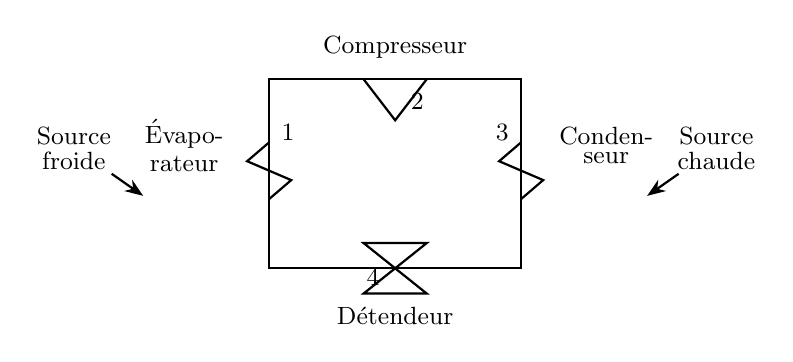
\begin{tikzpicture}[scale=0.8, >=Stealth, thick]
% boucle
\draw (0,0) -- (0,3) -- (4,3) -- (4,0) -- cycle;
% evaporateur
\draw (0,1.1) -- (0.35,1.4) -- (-0.35,1.7) -- (0,2.0);
\node at (-1.35,1.95) {\small\shortstack{Évapo-\\rateur}};
% condenseur
\draw (4,1.1) -- (4.35,1.4) -- (3.65,1.7) -- (4,2.0);
\node at (5.35,1.95) {\small\shortstack{Conden-\\seur}};
% compresseur
\draw (1.5,3) -- (2,2.35) -- (2.5,3);
\node at (2,3.5) {\small Compresseur};
% detendeur
\draw (1.5,0.4) -- (2.5,0.4) -- (2,0) -- cycle;
\draw (1.5,-0.4) -- (2.5,-0.4) -- (2,0) -- cycle;
\node at (2,-0.75) {\small Détendeur};
% sources
\node at (-3.1,1.9) {\small\shortstack{Source\\froide}};
\draw[->] (-2.5,1.5) -- (-2.0,1.15);
\node at (7.1,1.9) {\small\shortstack{Source\\chaude}};
\draw[->] (6.5,1.5) -- (6.0,1.15);
% points
\node at (0.3,2.15) {\small 1}; \node at (2.35,2.65) {\small 2};
\node at (3.7,2.15) {\small 3}; \node at (1.65,-0.15) {\small 4};
\end{tikzpicture}
\end{center}

\begin{center}
\renewcommand{\arraystretch}{1.5}
\begin{tabularx}{\linewidth}{@{}l l X@{}}
\toprule
\textbf{Étape} & \textbf{Transfo} & \textbf{Ce qui se passe} \\
\midrule
1 $\to$ 2 & Compression isentropique & vapeur BP $\to$ vapeur HP, $T$ et $p$ augmentent \\
2 $\to$ 3 & Condensation isobare (HP) & le fluide cède $Q_1<0$ à la source chaude, se liquéfie \\
3 $\to$ 4 & Détente isenthalpique ($h$=cste) & dans la soupape, $p$ et $T$ chutent, $W_{ut}=0$ et $Q=0$ \\
4 $\to$ 1 & Évaporation isobare (BP) & le fluide reçoit $Q_2>0$ de la source froide, se vaporise \\
\bottomrule
\end{tabularx}
\end{center}

\subsection{Le diagramme des frigoristes $(\log p,\,h)$}

En pratique on place le cycle sur un diagramme $\log p$ - $h$ du fluide (fourni à l'examen). Points \emph{réels}
notés $1',2',3',4'$ : on prévoit une \textbf{surchauffe} ($\sim5\,^\circ$C au-dessus de $T_{\text{évap}}$ en sortie
évaporateur, pour garantir un gaz sec avant le compresseur) et un \textbf{sous-refroidissement}
($\sim5\,^\circ$C sous $T_{cond}$ en sortie condenseur, pour garantir du liquide pur avant la soupape).

\begin{center}
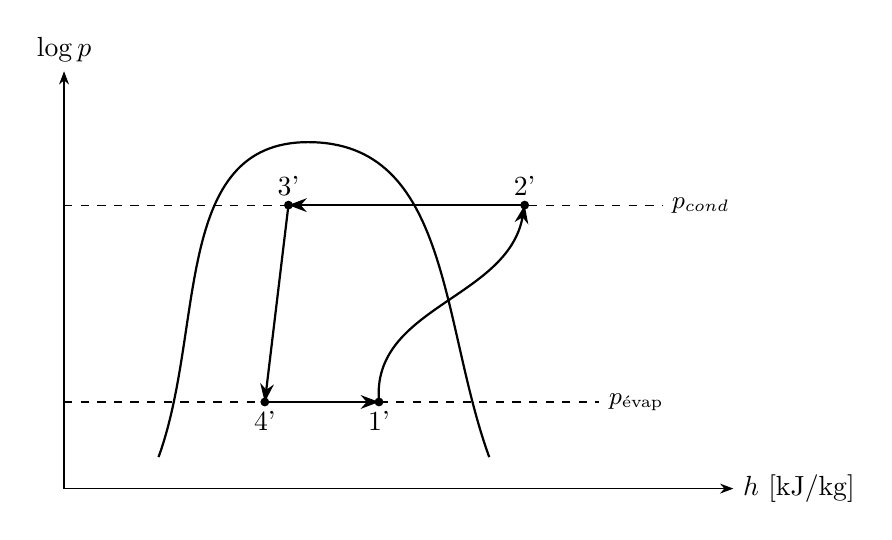
\begin{tikzpicture}[scale=1, >=Stealth]
\draw[->] (0,0) -- (8.5,0) node[right] {$h$ [kJ/kg]};
\draw[->] (0,0) -- (0,5.3) node[above] {$\log p$};
% dome
\draw[thick] (1.2,0.4) to[out=70,in=180] (3.1,4.4) to[out=0,in=110] (5.4,0.4);
% pressure levels
\draw[dashed] (0,3.6) -- (7.6,3.6) node[right]{\small $p_{cond}$};
\draw[dashed] (0,1.1) -- (6.8,1.1) node[right]{\small $p_{\text{évap}}$};
% points
\coordinate (p4) at (2.55,1.1); \coordinate (p1) at (4.0,1.1);
\coordinate (p2) at (5.85,3.6); \coordinate (p3) at (2.85,3.6);
\draw[thick,->] (p1) to[out=95,in=-100] (p2); % compression isentropique
\draw[thick,->] (p2) -- (p3); % condensation
\draw[thick,->] (p3) -- (p4); % détente isenthalpique
\draw[thick,->] (p4) -- (p1); % évaporation
\foreach \p/\lab/\pos in {p1/1'/below,p2/2'/above,p3/3'/above,p4/4'/below}
  {\fill (\p) circle (1.6pt) node[\pos] {\lab};}
\end{tikzpicture}
\end{center}

\begin{methode}
\textbf{Méthode pas à pas pour placer le cycle et lire les enthalpies}
\begin{enumerate}[leftmargin=1.6em]
\item Repérer sur l'axe vertical les deux pressions $p_{\text{évap}}$ (à $T_{\text{évap}}$) et $p_{cond}$ (à $T_{cond}$)
grâce à la cloche de saturation (intersection avec la courbe = pression de saturation à cette température).
\item Placer \textbf{1'} sur l'isobare $p_{\text{évap}}$, à $T_{\text{évap}}+$surchauffe (à droite de la cloche, en zone
vapeur).
\item Placer \textbf{2'} sur l'isobare $p_{cond}$, en suivant \textbf{l'isentropique} passant par 1'
(ou via $\eta_{isos}$ si compression non idéale, voir plus bas).
\item Placer \textbf{3'} sur l'isobare $p_{cond}$, à $T_{cond}-$sous-refroidissement (à gauche de la cloche,
zone liquide).
\item Placer \textbf{4'} \textbf{à la verticale de 3'} (même $h$, détente isenthalpique) sur l'isobare
$p_{\text{évap}}$.
\item Lire $h_{1'},h_{2'},h_{3'},h_{4'}$ directement sur l'axe des $h$.
\end{enumerate}
\end{methode}

\subsection{Formules}

\begin{center}
\renewcommand{\arraystretch}{1.7}
\begin{tabularx}{\linewidth}{@{}l X@{}}
\toprule
Travail compresseur (par kg) & $w=h_{2'}-h_{1'}$ \\
Chaleur cédée (condenseur, par kg) & $q_1=h_{3'}-h_{2'}$ \ (négatif) \\
Chaleur reçue (évaporateur, par kg) & $q_2=h_{1'}-h_{4'}$ \ (positif) \\
Vérification & $q_1+q_2+w=0$ \\
$PSN$ (frigo) & $PSN=\dfrac{Q_2}{W}=\dfrac{h_{1'}-h_{4'}}{h_{2'}-h_{1'}}$ \\
$COP$ (PAC) & $COP=\dfrac{-Q_1}{W}=\dfrac{h_{2'}-h_{3'}}{h_{2'}-h_{1'}}$ \\
Rendement isentropique du compresseur & $\eta_{isos}=\dfrac{h_{2isos}-h_1}{h_{2\,\text{réel}}-h_1}$ (donne
$h_{2'}$ réel à partir de $h_{2s}$ lu sur l'isentropique) \\
Bornes théoriques (Carnot, $T$ en K) & $COP_{max}=\dfrac{T_1}{T_1-T_2}$, \quad
$PSN_{max}=\dfrac{T_2}{T_1-T_2}$ \\
Débit de fluide frigorigène & $\dot m=\dfrac{P_{utile}}{|q_{utile}|}$ (kg/s), puis $P_{compresseur}=\dot m\cdot w$ \\
\bottomrule
\end{tabularx}
\end{center}

\begin{piege}
\textbf{$T_1$/$T_2$ dans les formules de Carnot = températures des \emph{sources}} (air extérieur, eau du
chauffage), \textbf{pas} les températures d'évaporation/condensation du fluide (qui sont décalées de
quelques degrés à cause de l'écart d'échange dans les échangeurs). Ne mélangez pas les deux dans une même
formule.
\end{piege}

\newpage
\subsection{Exemple complet résolu -- PAC au R134a pour le chauffage d'une maison}

\begin{enonce}
Une pompe à chaleur au R134a prélève de la chaleur à l'air extérieur pour chauffer l'eau d'un circuit de
radiateurs. Évaporation à $-5\,^\circ$C, condensation à $45\,^\circ$C, surchauffe et sous-refroidissement
de $5\,^\circ$C. Rendement isentropique du compresseur $\eta_{isos}=0{,}75$.

Lecture sur le diagramme $(\log p,h)$ du R134a : $h_{1'}=402{,}5$ kJ/kg ; $h_{2s}=435$ kJ/kg (point
isentropique) ; $h_{3'}=257$ kJ/kg.

La maison perd $P=12$ kW qu'il faut compenser. L'eau des radiateurs entre au condenseur à $35\,^\circ$C
et en ressort à $40\,^\circ$C ($c_{eau}=4185$ J/kg·K).

\emph{Trouver : le COP de la PAC, le débit de R134a, la puissance du compresseur, et le débit d'eau du
circuit de chauffage.}
\end{enonce}

\begin{correction}
\textbf{1) Point 2' réel (compression non isentropique)} :
\[\eta_{isos}=\frac{h_{2s}-h_{1'}}{h_{2'}-h_{1'}} \Rightarrow
h_{2'}=h_{1'}+\frac{h_{2s}-h_{1'}}{\eta_{isos}}=402{,}5+\frac{435-402{,}5}{0{,}75}=402{,}5+43{,}3
=445{,}8\text{ kJ/kg}\]

\textbf{2) Point 4'} (détente isenthalpique) : $h_{4'}=h_{3'}=257$ kJ/kg.

\textbf{3) Énergies échangées par kg de fluide} :
\[w=h_{2'}-h_{1'}=445{,}8-402{,}5=43{,}3\text{ kJ/kg}\]
\[q_1=h_{3'}-h_{2'}=257-445{,}8=-188{,}8\text{ kJ/kg} \ \ (\Rightarrow |q_1|=188{,}8\text{ kJ/kg})\]
\[q_2=h_{1'}-h_{4'}=402{,}5-257=145{,}5\text{ kJ/kg}\]
\emph{Vérification : } $q_1+q_2+w=-188{,}8+145{,}5+43{,}3\approx0$ \checkmark

\textbf{4) COP de la PAC} :
\eqbox{COP=\frac{-q_1}{w}=\frac{188{,}8}{43{,}3}=\mathbf{4{,}36}}

\emph{Comparaison Carnot (source froide $=-5\,^\circ$C$=268{,}15$K, source chaude $=45\,^\circ$C$=318{,}15$K)} :
$COP_{max}=\dfrac{318{,}15}{318{,}15-268{,}15}=6{,}36$. Notre COP réel ($4{,}36$) représente $\sim69\%$
du maximum théorique, ce qui est réaliste pour une PAC.

\textbf{5) Débit de fluide frigorigène} (le condenseur doit fournir $12$ kW) :
\eqbox{\dot m_{R134a}=\frac{P}{|q_1|}=\frac{12}{188{,}8}=\mathbf{0{,}0636\ kg/s}}

\textbf{6) Puissance du compresseur} :
\eqbox{P_{comp}=\dot m_{R134a}\cdot w=0{,}0636\times43{,}3=\mathbf{2{,}76\ kW}}

\emph{(Vérification cohérence : $P_{comp}+P_{\text{évap}}=P_{cond}$, soit $2{,}76+\dot m\cdot q_2=2{,}76+
0{,}0636\times145{,}5=2{,}76+9{,}25=12{,}0$ kW \checkmark)}

\textbf{7) Débit d'eau du circuit de chauffage} -- échangeur ouvert isobare, $\Delta H=Q$ :
\[P=\dot m_{eau}\cdot c_{eau}\cdot\Delta T \Rightarrow
\dot m_{eau}=\frac{P}{c_{eau}\cdot\Delta T}=\frac{12\,000}{4185\times5}\]
\eqbox{\dot m_{eau}\approx \mathbf{0{,}573\ kg/s}\ (\approx2{,}06\ \text{m}^3/\text{h})}
\end{correction}

\begin{piege}
La partie « échange thermique » (eau du chauffage, air d'un local, etc.) se traite \textbf{toujours} avec
$P=\dot m\, c\,\Delta T$ (ou $Q=mc\Delta T$ sans débit) -- c'est simplement le 1\textsuperscript{er} principe
en système ouvert isobare ($\Delta H=Q$) appliqué à un fluide \emph{sans} changement de phase. Le lien entre
les deux circuits (fluide frigorigène $\leftrightarrow$ eau) se fait via la \textbf{puissance échangée},
identique des deux côtés de l'échangeur.
\end{piege}

\newpage
\section{Exercices d'entraînement corrigés}

\noindent\textit{Essayez de résoudre chaque exercice seul (avec le formulaire) avant de lire la correction.
Les 4 exercices couvrent les 3 types qui reviennent le plus souvent à l'examen : cycle moteur/turbine à gaz,
moteur à piston (diesel, 2 temps), et cycle frigorifique.}

\subsection{Exercice 1 -- Cycle moteur à turbine à gaz (double détente)}

\begin{enonce}
On observe un cycle moteur utilisant de l'air (gaz parfait, $c_p=1004$ J/kg·K, $\gamma=1{,}4$), débit
massique $\dot m=35$ kg/s :
\begin{itemize}[leftmargin=1.4em,itemsep=1pt]
\item 1-2 : compression adiabatique réversible de 1 atm à 4,1 atm ; $T_1=15\,^\circ$C.
\item 2-3 : échauffement isobare jusqu'à $T_3=750\,^\circ$C.
\item 3-4 : détente adiabatique réversible dans une 1\textsuperscript{ère} turbine ; $p_4$ inconnue, mais
tout le travail de cette turbine sert uniquement à entraîner le compresseur (1-2).
\item 4-5 : échauffement isobare jusqu'à $T_5=700\,^\circ$C.
\item 5-6 : détente adiabatique réversible dans une 2\textsuperscript{nde} turbine, jusqu'à $p_6=p_1$.
\item 6-1 : refroidissement isobare (fermeture du cycle).
\end{itemize}
\emph{Trouver : $T_2,T_4,T_6$ et $p_4$ ; le rendement du cycle ; la puissance utile de la 2\textsuperscript{nde}
turbine.}
\end{enonce}

\begin{correction}
\textbf{Point 2} (compression adiabatique, $T_1=288{,}15$ K) :
\[T_2=T_1\left(\frac{p_2}{p_1}\right)^{\frac{\gamma-1}{\gamma}}=288{,}15\times4{,}1^{0{,}2857}
=\mathbf{431{,}2\text{ K}}\]

\textbf{Point 4} : le travail de la turbine 1 égale (en valeur absolue) celui du compresseur, avec le même
débit dans les deux : $c_p(T_3-T_4)=c_p(T_2-T_1)\Rightarrow T_3-T_4=T_2-T_1$.
Avec $T_3=1023{,}15$ K :
\[T_4=T_3-(T_2-T_1)=1023{,}15-(431{,}2-288{,}15)=\mathbf{880{,}1\text{ K}}\]

\textbf{Pression $p_4$} (adiabatique 3-4) : $\dfrac{T_4}{T_3}=\left(\dfrac{p_4}{p_2}\right)^{0{,}2857}$
\[p_4=p_2\left(\frac{T_4}{T_3}\right)^{1/0{,}2857}=4{,}1\times\left(\frac{880{,}1}{1023{,}15}\right)^{3{,}5}
=\mathbf{2{,}42\text{ atm}}\]

\textbf{Point 6} (adiabatique 5-6, $T_5=973{,}15$ K, jusqu'à $p_6=p_1=1$ atm) :
\[T_6=T_5\left(\frac{p_1}{p_4}\right)^{0{,}2857}=973{,}15\times\left(\frac{1}{2{,}42}\right)^{0{,}2857}
=973{,}15\times0{,}7769=\mathbf{756{,}0\text{ K}}\]

\textbf{Rendement.} Chaleur reçue (2-3 et 4-5, isobares) :
\[q_{23}=c_p(T_3-T_2)=1004\times591{,}93=594{,}3\text{ kJ/kg}\qquad
q_{45}=c_p(T_5-T_4)=1004\times93{,}07=93{,}4\text{ kJ/kg}\]
\[Q_{in}=q_{23}+q_{45}=\mathbf{687{,}7\text{ kJ/kg}}\]
Seul le travail de la 2\textsuperscript{nde} turbine est net (celui de la 1\textsuperscript{ère} est
entièrement consommé par le compresseur) :
\[|W_{net}|=c_p(T_5-T_6)=1004\times(973{,}15-756{,}0)=218{,}0\text{ kJ/kg}\]
\eqbox{\eta=\frac{|W_{net}|}{Q_{in}}=\frac{218{,}0}{687{,}7}=\mathbf{31{,}7\%}}

\textbf{Puissance utile de la 2\textsuperscript{nde} turbine} (convention : travail \emph{fourni par} le
fluide $\Rightarrow$ négatif) :
\eqbox{P=-\dot m\cdot|W_{net}|=-35\times218{,}0=\mathbf{-7{,}63\ MW}}
\end{correction}

\subsection{Exercice 2 -- Moteur diesel 4 cylindres}

\begin{enonce}
Moteur diesel 4 temps, 4 cylindres, cylindrée totale 2 L ($0{,}5$ L/cylindre). Rapport volumétrique
$\varepsilon=18$, rapport de combustion $\rho=2$. Air admis à $27\,^\circ$C, 1 bar, $\gamma=1{,}4$,
$R=8{,}314$ J/mol·K. Vitesse de rotation $N=2200$ tr/min.

\emph{Trouver $T,p,V$ en B, C, D, E ; le rendement théorique ; la chaleur $Q_{CD}$ et le travail théorique
par cylindre et par cycle ; la puissance théorique du moteur.}
\end{enonce}

\begin{correction}
\textbf{Volumes.} $V_B-V_A=500\text{ cm}^3$, $\varepsilon=V_B/V_A=18\Rightarrow V_A=V_C=29{,}4\text{ cm}^3$,
$V_B=529{,}4\text{ cm}^3$. Combustion isobare : $V_D=\rho V_C=58{,}8\text{ cm}^3$.

\textbf{B} : $T_B=300{,}15$ K, $p_B=1$ bar.

\textbf{C} (compression adiabatique) :
\[T_C=T_B\,\varepsilon^{\gamma-1}=300{,}15\times18^{0{,}4}=\mathbf{953{,}7\text{ K}}\qquad
p_C=p_B\,\varepsilon^\gamma=18^{1{,}4}=\mathbf{57{,}2\text{ bar}}\]

\textbf{D} (combustion isobare, $p_D=p_C$) : $T_D=T_C\cdot\rho=953{,}7\times2=\mathbf{1907{,}4\text{ K}}$

\textbf{E} (détente adiabatique jusqu'à $V_E=V_B$, soit $V_D/V_E=\rho/\varepsilon=1/9$) :
\[T_E=T_D\left(\frac{1}{9}\right)^{0{,}4}=\mathbf{792{,}2\text{ K}}\qquad
p_E=p_D\left(\frac{1}{9}\right)^{1{,}4}=\mathbf{2{,}64\text{ bar}}\]

\textbf{Rendement théorique} :
\[\eta_{\text{théo}}=1-\frac{1}{\varepsilon^{\gamma-1}}\cdot\frac{\rho^\gamma-1}{\gamma(\rho-1)}
=1-\frac{1}{3{,}178}\times\frac{2^{1{,}4}-1}{1{,}4\times1}=1-0{,}3147\times1{,}171\]
\eqbox{\eta_{\text{théo}}=\mathbf{63{,}2\%}}

\emph{Remarque : c'est exactement la formule du formulaire
$\eta=1+\dfrac{\varepsilon^{1-\gamma}-\varepsilon^{1-\gamma}\rho^{\gamma}}{\gamma(\rho-1)}$, simplement
réarrangée en mettant $\varepsilon^{1-\gamma}=\frac{1}{\varepsilon^{\gamma-1}}$ en facteur. Utilisez celle
que vous préférez, elles donnent le même nombre.}

\textbf{Chaleur apportée} (isobare, $n=\dfrac{p_BV_B}{RT_B}=\dfrac{10^5\times529{,}4\times10^{-6}}
{8{,}314\times300{,}15}=0{,}02123$ mol, $C_p=\dfrac{\gamma R}{\gamma-1}=29{,}1$ J/mol·K) :
\[Q_{CD}=nC_p(T_D-T_C)=0{,}02123\times29{,}1\times953{,}7=\mathbf{589\text{ J}}\ \text{(par cylindre, par cycle)}\]

\textbf{Travail théorique} : $|W_{\text{théo}}|=\eta_{\text{théo}}\cdot Q_{CD}=0{,}632\times589=\mathbf{372\text{ J}}$

\textbf{Puissance théorique} ($z=4$, 1 cycle = 2 tours) :
\eqbox{P_{th}=\frac{N}{2\cdot60}\cdot|W_{\text{théo}}|\cdot z=\frac{2200}{120}\times372\times4
=\mathbf{27{,}3\ kW}}
\end{correction}

\subsection{Exercice 3 -- Petit moteur 2 temps}

\begin{enonce}
Petit moteur 2 temps monocylindre, $\varepsilon=9$, $\gamma=1{,}4$. La combustion apporte $Q_{CD}=80$ J par
cycle. Rendement de forme $\eta_f=0{,}70$, rendement mécanique $\eta_{\text{méca}}=0{,}85$.
Vitesse de rotation $N=4000$ tr/min.

\emph{Trouver le rendement théorique, le travail disponible par cycle, et la puissance effective.}
\end{enonce}

\begin{correction}
\textbf{Rendement théorique} (même formule que l'essence 4 temps, seule la mécanique de renouvellement
du mélange change) :
\eqbox{\eta_{\text{théo}}=1-\varepsilon^{1-\gamma}=1-9^{-0{,}4}=1-0{,}4153=\mathbf{58{,}5\%}}

\textbf{Travaux en cascade} :
\[|W_{\text{théo}}|=\eta_{\text{théo}}\cdot Q_{CD}=0{,}585\times80=46{,}8\text{ J}\]
\[|W_{\text{indiqué}}|=\eta_f\cdot|W_{\text{théo}}|=0{,}70\times46{,}8=32{,}8\text{ J}\]
\[|W_{disponible}|=\eta_{\text{méca}}\cdot|W_{\text{indiqué}}|=0{,}85\times32{,}8=\mathbf{27{,}8\text{ J}}\]

\textbf{Puissance effective} -- \textbf{attention} : en 2 temps, 1 tour = 1 cycle, donc pas de
$\div 2$ :
\eqbox{P_{eff}=\frac{N}{60}\cdot|W_{disponible}|\cdot z=\frac{4000}{60}\times27{,}8\times1
=\mathbf{1{,}85\ kW}}
\end{correction}

\begin{piege}
C'est l'erreur la plus fréquente sur cette matière : garder le $\div 2\cdot 60$ du 4 temps pour un moteur
2 temps. Relisez toujours l'énoncé : « 1 tour = 1 cycle » (2 temps) ou « 1 cycle = 2 tours » (4 temps).
\end{piege}

\subsection{Exercice 4 -- Cycle frigorifique au NH\textsubscript{3}}

\begin{enonce}
Une machine frigorifique fonctionne au NH$_3$ (ammoniac). Évaporation à $-10\,^\circ$C, condensation à
$50\,^\circ$C, surchauffe et sous-refroidissement de $5\,^\circ$C chacun.

\emph{Placez le cycle sur le diagramme $(\log p,h)$ du NH$_3$ (fourni à l'examen), trouvez les enthalpies
de chaque point, puis la $PSN$.}
\end{enonce}

\begin{correction}
\textbf{Méthode} (voir section 2.2) : on repère $p_{\text{évap}}$ (isobare à $-10\,^\circ$C) et $p_{cond}$ (isobare
à $50\,^\circ$C) sur la cloche de saturation du NH$_3$.
\begin{itemize}[leftmargin=1.4em]
\item \textbf{1'} : sur l'isobare basse pression, à $-10+5=-5\,^\circ$C (zone vapeur, à droite de la
cloche).
\item \textbf{2'} : sur l'isobare haute pression, en suivant l'isentropique passant par 1'.
\item \textbf{3'} : sur l'isobare haute pression, à $50-5=45\,^\circ$C (zone liquide, à gauche de la cloche).
\item \textbf{4'} : à la verticale de 3' (même $h$), sur l'isobare basse pression.
\end{itemize}

\emph{Valeurs indicatives lues sur le diagramme (elles varient selon la précision de votre tracé -- l'ordre
de grandeur et la méthode comptent) :}
\[h_{1'}\approx1760\text{ kJ/kg}\qquad h_{2'}\approx2050\text{ kJ/kg}\qquad
h_{3'}=h_{4'}\approx700\text{ kJ/kg}\]

\textbf{PSN} :
\eqbox{PSN=\frac{Q_2}{W}=\frac{h_{1'}-h_{4'}}{h_{2'}-h_{1'}}=\frac{1760-700}{2050-1760}
=\frac{1060}{290}=\mathbf{3{,}66}}

\emph{Interprétation : pour 1 kWh de travail de compression fourni, on extrait $\approx3{,}66$ kWh à la
source froide -- c'est pour cela qu'une machine frigorifique/PAC est plus efficace qu'un chauffage
électrique direct (qui a un « rendement » de 1).}
\end{correction}

\begin{methode}
\textbf{Ce qu'il faut absolument savoir refaire sans le cours} pour les 3 exercices récurrents annoncés
(gaz réfrigérant type R134a, frigo/chauffage avec échange thermique, moteur essence/diesel/2 temps) :
\begin{enumerate}[leftmargin=1.6em]
\item Construire le tableau d'état et identifier chaque transformation (section 1).
\item Placer un cycle frigo sur un diagramme $(\log p,h)$ et en tirer $PSN$/$COP$ (section 2).
\item Dériver $\eta_{\text{théo}}$ à partir de $\varepsilon$ (et $\rho$) pour un moteur, \emph{sans} passer par
la combustion (section 1).
\item Relier un cycle fermé (cylindre, fluide frigorigène) à un circuit ouvert externe (eau de chauffage,
air ambiant) via la puissance échangée et $Q=\dot m\,c\,\Delta T$.
\end{enumerate}
\end{methode}


\end{document}
